\documentclass[12pt]{article}
\usepackage[margin=40pt]{geometry}
\usepackage[utf8]{inputenc}
\usepackage{babel}
\usepackage[T1]{fontenc}

\usepackage{fancyvrb}
\usepackage{multicol}
\usepackage{graphicx}
\usepackage{fancyvrb}
\usepackage{url}
\graphicspath{ {./images/} }

\title{\Huge Dopplerov jav}
\author{Adam Labuš, Sexta B}

\def\ruler{%
	\vspace{0.5em}
	\noindent\rule{\textwidth}{0.5pt}
	\vspace{0.5em}
}

\begin{document}
	\maketitle

	\tableofcontents

	\section{Opis}
	Dopplerov jav nastáva, keď sa pozorovateľ hýbe relatívne ku zdroju alebo zdroj vlnenia sa hýbe relatívne ku pozorovateľovi, alebo obidve naraz. 
Najčastejšie sa s ním stretávame v meste, kde pri prechode auta so sírenami (zdroj zvuku/vlnenia) je počuť zmenu tónu sirény potom ako okolo nás prejde.Konkrétne keď sa zdroj vlnenia ku nám približuje tak počujeme vyšší tón, naopak keď sa od nás vzďaluje tak počujeme nižší tón.
	\footnote{\url{https://en.wikipedia.org/wiki/File:Speeding-car-horn_doppler_effect_sample.ogg}}
	Nakoľko svetlo je tiež len vlnenie vieme toto pozorovať aj pri svetle z hviezd, ktoré mení farbu podľa relatívnej rýchlosti hviezdy voči našej planéte, podľa čoho vieme povedať, že sa od nás vzďalujú.
	\footnote{\url{https://www.youtube.com/watch?v=h4OnBYrbCjY}}

	\begin{center}
		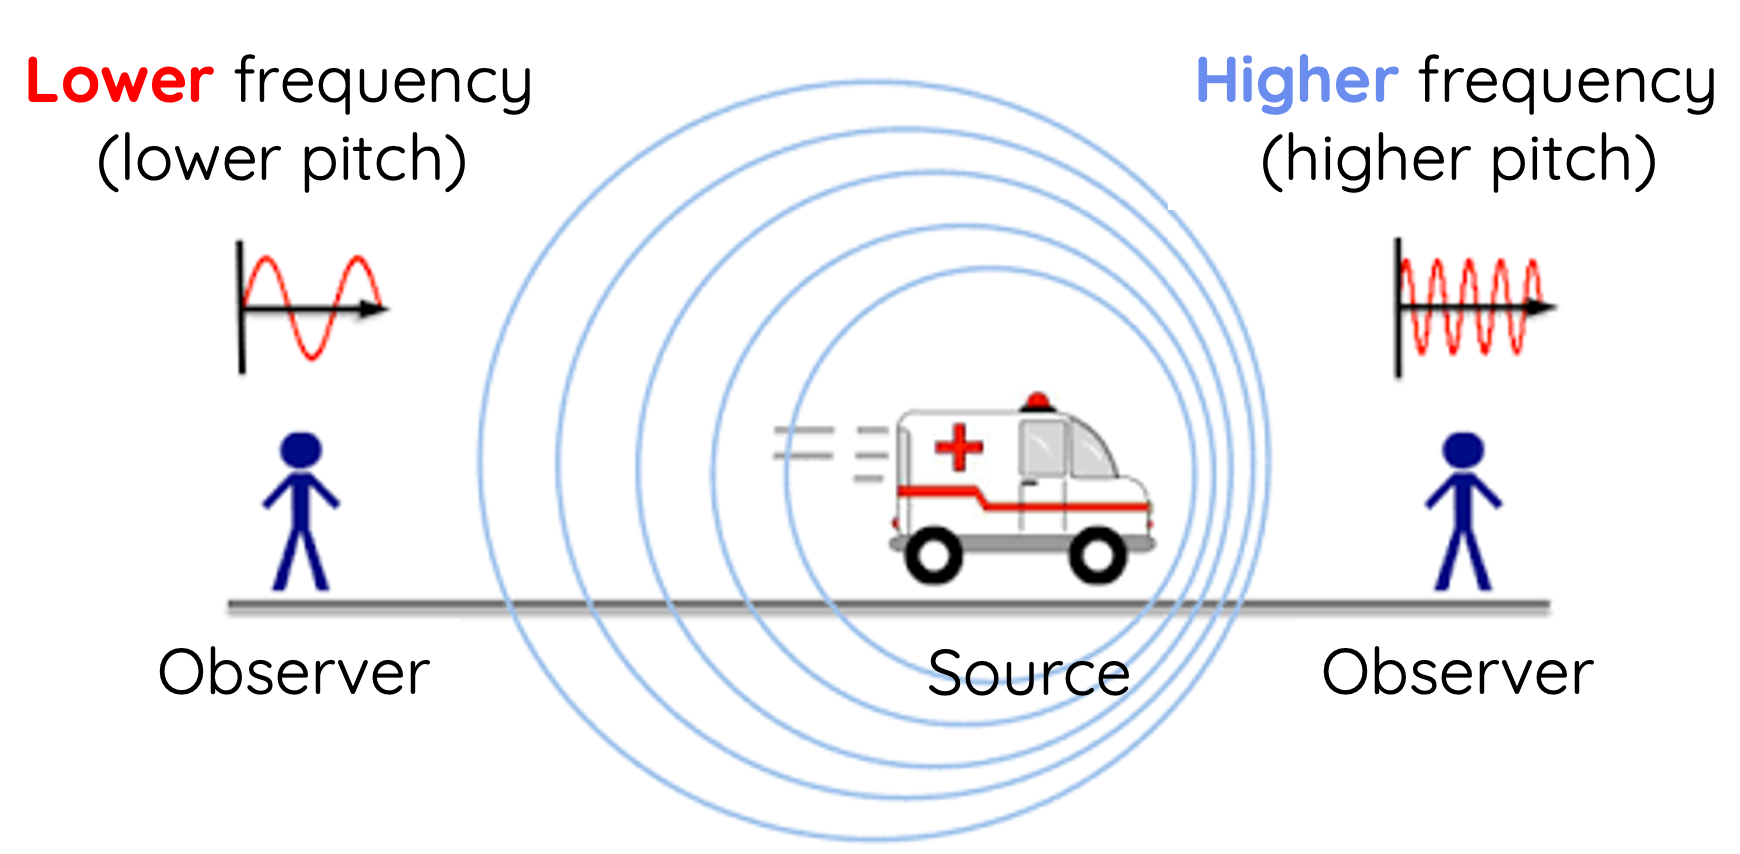
\includegraphics[width=.5\textwidth]{simple_explanation}
	\end{center}

	Na ľavej strane obrázku vidíme prípad stacionárneho pozorovateľa od ktorého sa vzdaľuje zdroj vlnenia a na pravom je prípad stacionárneho pozorovateľa ku ktorému sa približuje zdroj vlnenia. Pozorovateľ na ľavej strane počuje zvuk ako nižší tón (menšia frekvencia) ako je pri zdroji a pozorovateľ počuje zvuk ako vyšší tón (vyššia frekvencia) ako je pri zdroji. 

	\newpage
	\section{Výpočty}

	Ak je pozorovateľ stacionárny a zdroj vlnenia pohyblivý:\\[1em]
	$f = f_0\frac{v}{v + v_{s,r}}$\\[1em]
	Ak je pozorovateľ pohyblivý a zdroj vlnenia stacionárny:\\[1em]
	$f = f_0(1 + \frac{v}{v + v_{r,s}})$\\
	\begin{itemize}
		\item $f$ = frekvencia vlnenia pri pozorovateľovi
		\item $f_0$ = frekvencia vlnenia pri zdroji
		\item $v$ = rýchlosť propagácie vlnenia v danej látke
		\item $v_{s,r}$ = relatívna rýchlosť zdroja voči pozorovateľovi\\
		$v_{s,r} < 0$ => zdroj sa približuje\\
		$v_{s,r} > 0$ => zdroj sa vzďaluje\\
		\item $v_{r,s}$ = relatívna rýchlosť zdroja pozorovateľova voči zdroju\\
			$v_{r,s} < 0$ => pozorovateľ sa približuje\\
			$v_{r,s} > 0$ => pozorovateľ sa vzďaluje\\
	\end{itemize}


	\footnote{\url{http://kf-lin.elf.stuba.sk/~ballo/STU_online/Fyzika I/VI kapitola/kmity-vlny2-8.htm}}
\end{document}
